% LTeX: language=fr enabled=true

\chapter{Modélisation et commande d'un drone à aile libre rotation libre}
\minitoc
\label{chap:colibri}

\section{Motivation}
\label{sec:motivationcolibri}
Les nombreux avantages d'une architecture tailsitter nous ont poussé à nous intéresser à leurs stabilisations. Nous avons toutefois observé une limitation dans leur usage. Effectivement, l'aile change d'incidence en fonction de la vitesse du drone ou du vent environnent et toute charge utile se trouve en rotation avec l'aile, ce qui est inapproprié pour une caméra ou une sonde Pitot qui doivent pouvoir maintenir une direction constante. Ainsi, nous avons pensé à une nouvelle architecture, a mi-chemin entre un \textit{tailsitter} et un \textit{tiltwing}, appelé \textit{freewing}. Cette dernière conserve les avantages du \textit{tiltwing} en ce qu'elle permet d'avoir un fuselage que l'on peut maintenir constamment horizontal. Elle s'inspire des \textit{tailsitters} en permettant de modifier librement l'incidence de l'aile pour se désensibiliser des turbulences. L'aile étant libre de s'orienté vis-à-vis du fuselage, une augmentation de portance engendré par une augmentation de la vitesse du flux d'air (turbulence) modifiera l'angle d'incidence de l'aile ce qui engendrera une diminution de la portance et donc un nouvel équilibre.

De plus, le fuselage permettra l'emport d'une charge utile fragile car il pourra être maintenu horizontal en toute circonstance. Mais aussi permettre d'emporter des capteurs et la batterie. L'ensemble de la masse du drone sera concentré sur le fuselage de manière à minimiser l'inertie de l'aile et facilité sa rotation face à des turbulences faibles.

\section{Design et modélisation d'un drone : Colibri}
\label{sec:model_colibri}

Le drone Colibri est dérivé d'un drone \textit{tailsitter} qui génère de la portance pendant le vol d'avancement. Cette aile possède plusieurs actionneurs : quatre moteurs $u_{i}, ~i = 1,2,3,4$ et deux élevons $\delta_{\text{l}}$ et $\delta_{\text{r}}$. Nous pouvons définir le vecteur de contrôle $u_{\text{W}}$ de l'aile d'après la Figure~\ref{fig:world_body} comme $u_{\text{W}} = [u_{1}~u_{2}~u_{3}~u_{4}~\delta_{\text{l}}~\delta_{\text{r}}]^\top$. Un fuselage relié par un pivot est fixé au centre aérodynamique de l'aile. Ce fuselage supporte l'autopilote, la batterie, un moteur et un empennage pour le maintenir horizontal.

Dans la Figure~\ref{fig:world_body}, toutes les surfaces de contrôle aérodynamiques sont représentées en rose et les hélices en vert. Trois repères sont attachés au drone tel que : (I) est un repère inertiel NED lié à la surface de la terre, (W) est un repère attaché à l'aile du drone et (F) est un repère attaché au fuselage du drone.



\begin{figure}[ht!]
\centering
    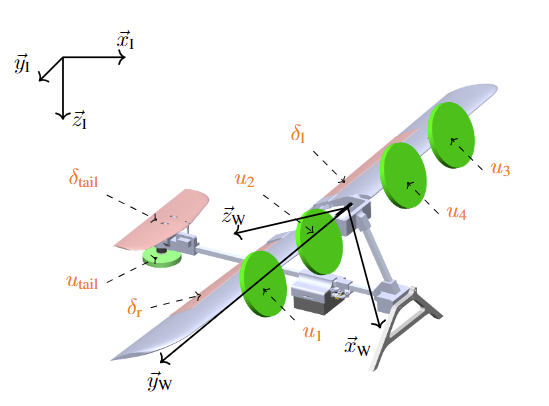
\includegraphics[width=0.6\columnwidth,angle=0,trim={0 0 0 0.5cm},clip]{figures/wold_body.png}
    \caption{Les repères, inertiel (I) et aile (W), attachés à l'architecture de Colibri.}
    \label{fig:world_body}
\end{figure}

Certaines des dimensions caractéristiques sont indiquées dans la Table~\ref{tab:pars_colibri}. Notons que les moteurs sont positionnés symétriquement sur l'aile, ce qui signifie que la position peut être décrite en se concentrant sur un seul côté. 

\begin{table}[ht]
  \centering
    \begin{tabular}{|l|c|c|}
      \hline
      \multicolumn{1}{|c|}{Paramètres} & Valeur & Unités  \\
      \hline
      $m_{\text{W}}$ (masse de l'aile)  & 0.53& \SI{}{\kilogram} \\
      \hline
      $m_{\text{F}}$ (masse du fuselage)  & 1.17& \SI{}{\kilogram} \\
      \hline
    %   $b$ (wingspan)  & 1.17 & \SI{}{\meter} \\
    %   \hline
    %   $c$ (aerodynamic cord)  & 0.150 & \SI{}{\meter} \\
    %   \hline
    %   $S$ (wing area) & 0.1537 & \SI{}{\square\meter}\\
    %   \hline
    %   $S_{\text{wet}}$ (wet area) & 0.0813 & \SI{}{\square\meter}\\
    %   \hline
    %   $S_{\text{p}}$ (propeller area) & 0.0182 & \SI{}{\square\meter}\\
    %   \hline
      $J_{\text{W}}=diag(J_{x}^{\text{W}}, J_{y}^{\text{W}}, J_{z}^{\text{W}})$ & \!\! $\diag(0.1677,0.0052,0.1634)$\!\! & \SI{}{\kilogram\square\meter}\\
      \hline
      $J_{\text{F}}=diag(J_{x}^{\text{F}}, J_{y}^{\text{F}}, J_{z}^{\text{F}})$ & \!\! $\diag(0.0191,0.0161,0.0343)$\!\! & \SI{}{\kilogram\square\meter}\\
      \hline
      $k_{\text{f}}$ (coefficient de poussée de l'hélice) & 1.7800e-8 & \SI{}{\kilogram\meter}\\
      \hline
       $d_{\text{M}O_{\text{W}}}$  & $[0.383,0,-0.167]^\top$ & \SI{}{\meter}\\
      \hline
       $d_{\text{G}O_{\text{W}}}$  & $[0.052,0,-0.171]^\top$ & \SI{}{\meter}\\
      \hline
    \end{tabular}
    \caption{Paramètres numériques du modèle Colibri.}
    \label{tab:pars_colibri}
\end{table}


La modélisation est basée sur les résultats de \cite[Section 2.15]{udwadia-phohomsiri}. L'algorithme de calcul des matrices $M$, $A$, $Q$ et $B$ se trouve dans \cite{udwadia-schutte}, qui nous fournit les équations de mouvement d'un système multicorps contraint : 
\begin{align}
\label{eq:udwadia}
    \ddot{x} = \hat{M}^{\dag} \begin{bmatrix} Q \\ B \end{bmatrix}  = \begin{bmatrix} (I - A^{\dag}A)M \\ A \end{bmatrix}^{\dag} \begin{bmatrix} Q \\ B \end{bmatrix}
\end{align}
dont l'expression est valide tant que $\hat{M}$ a un rang complet et où $A$, $M$, $Q$ et $B$ sont décrits par la suite.

\begin{figure}[ht!]
    \centering
    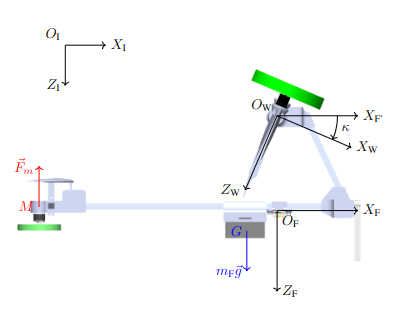
\includegraphics[width=0.6\columnwidth,angle=0,trim={0 0 0 0.5cm},clip]{figures/fram_side_colibri.png}
    \caption{Repère inertiel (I), du fuselage (F) et de l'aile (W) et forces agissant sur le drone Colibri.}
    \label{fig:colibri_frame_side}
\end{figure}
Nous utiliserons les quaternions $q = \left[ \eta ~ \epsilon^\top \right]^\top  \in {\mathbb S}^3:=\{ q\in \real^4: |q| = 1\}$ pour représenter les orientations des deux corps. La matrice de rotation qui en résulte $R(q) \in SO(3): = \{R\in \real^{3\times 3}: R^\top R = I,~\det(R)=1\}$ est définie de manière unique comme $R(q) := I +2\eta \skewsym{\epsilon} + 2\skewsym{\epsilon}^{2} = [R_{1}~R_{2}~R_{3}]$.

D'après les Figures~\ref{fig:world_body} et \ref{fig:colibri_frame_side}, nous définissons les vecteurs $p_{\text{F}} = \overrightarrow{O_{\text{I}} O_{\text{F}}} $, $p_{\text{W}} = \overrightarrow{O_{\text{I}} O_{\text{W}}} $, $d_{\text{FW}} = \overrightarrow{O_{\text{F}} O_{\text{W}}} $ satisfaisant $d_{\text{FW}} = p_{\text{W}} - p_{\text{F}}$ and $d_{\text{M}O_{\text{W}}} = \overrightarrow{\text{M} O_{\text{W}} }$, $d_{\text{G}O_{\text{W}}} = \overrightarrow{\text{G} O_{\text{W}} }$.

D'après \cite{Tangirala2015}, nous avons une définition d'une réalisation minimale : 
\begin{definition}[Réalisation minimale]
    \label{def:reaMini}
    Une réalisation est dite "minimale" si elle décrit le système avec le nombre minimum d'états. Le nombre minimum de variables d'état nécessaire pour décrire un système est égal à l'ordre de l'équation différentielle.
\end{definition}


Le vecteur d'état global est $(x,v) \in \real^{28}$ avec $x=(p_{\text{W}},~q_{\text{W}},~p_{\text{F}},~q_{\text{F}}) \in \real^{14}$ et $v=(v_{\text{W}},~\dot{q}_{\text{W}},~v_{\text{F}},~\dot{q}_{\text{F}}) = (\dot{p}_{\text{W}},~\dot{q}_{\text{W}},~\dot{p}_{\text{F}},~\dot{q}_{\text{F}})=\dot{x} \in \real^{14}$. Nous avons $v_{\text{W}} = \dot{p}_{\text{W}} \in \real^{3}$ qui représente la vitesse linéaire de l'aile dans le repère inertiel ; $\dot{q}_{\text{W}} \in \real^{4}$  est la dérivée du quaternion. $q_{\text{W}} \in \real^{4}$ représentant l'orientation de l'aile ; $v_{\text{F}} =p_{\text{F}} \in \real^{3}$  est la vitesse linéaire du fuselage dans le repère inertiel et $\dot{q}_{\text{F}} \in \real^{4}$  est la dérivée du quaternion. $q_{\text{F}} \in \real^{4}$ représentant l'orientation du fuselage. Nous observons que le vecteur d'état n'est pas minimal d'après la définition \ref{def:reaMini}. Effectivement, le système possède sept degrés de liberté (six degrés pour l'aile et un degré pour le fuselage) et nous le représentons avec un vecteur d'état de dimension quatorze.

Il convient de noter que la vitesse angulaire $\omega \in \real^{3}$ peut être obtenue à partir de la dérivée du quaternion $\dot{q}$ en utilisant l'équation \cite[équation (2.7)]{udwadia-schutte} rappelée ici : 
\begin{align*}
    \omega = H(q) \dot{q} 
\end{align*}
où $H(q) \in \real^{3\times4}$ est une matrice définie par $H(q) = 2\begin{bmatrix}-\epsilon & \eta I_{3} - \skewsym{\epsilon}\end{bmatrix}$.
Pour dériver les équations du mouvement, rappelons que  $R_{i}(q) \in \real^{3}, i = 1,2,3$ sont les trois colonnes d'une matrice de rotation associée au quaternion $q$, lequelles définissent les matrices $L_{\text{i}}^{\text{W}} \left( q_{\text{W}} \right) = \frac{\partial R_{i}}{\partial q}(q_{\text{W}}) \in \real^{3\times4}$, 
$L_{\text{i}}^{\text{F}} \left( q_{\text{F}} \right) = \frac{\partial R_{i}}{\partial q}(q_{\text{F}}) \in \real^{3\times4}$ et
$L_{O_{\text{F}}^{\text{W}}} = \sum_{i=1}^{3} d_{\text{FW}}(i) L_{\text{i}}^{\text{F}} (q_{\text{F}})$, $i \in {1,2,3}$, où $d_{\text{FW}}(i)$ désigne la i-ème composante du vecteur $d_{\text{FW}} = p_{\text{W}} - p_{\text{F}}$. Comme $O_{\text{W}}$ est situé au centre de rotation de l'aile, la distance $d_{\text{FW}}$ est une constante, puisque $O_{\text{W}}$ et $O_{\text{F}}$ appartiennent au même solide (le fuselage).

On en déduit, avec homogénéité, $\dot{L}_{O_{\text{F}}^{\text{W}}} = \sum_{i=1}^{3} d_{\text{FW}}(i) L_{\text{i}}^{\text{F}} (\dot{q}_{\text{F}})$. Avec ces définitions, les matrices de \eqref{eq:udwadia} sont :

% \todo{There is no derived process or explanation provided for
% the M matrix, A, Q matrix, etc. In Equation 1, both Q and B
% are matrices and do not include the location x. Where are
% the state variables located?}

\begin{align}
    M = \begin{bmatrix}
        m_{\text{W}} I_{3} & \mathbb{0}_{3 \times 4} & \mathbb{0}_{3} & \mathbb{0}_{3 \times 4}\\
        \mathbb{0}_{4 \times 3} & H_{\text{W}}^\top J_{\text{W}} H_{\text{W}} & \mathbb{0}_{4 \times 3} & \mathbb{0}_{4}\\
        \mathbb{0}_{3} & \mathbb{0}_{3 \times 4} & m_{\text{F}} I_{3} & \mathbb{0}_{3 \times 4} \\
        \mathbb{0}_{4 \times 3} & \mathbb{0}_{4 } & \mathbb{0}_{4 \times 3} & H_{\text{F}}^\top J_{\text{F}} H_{\text{F}}    \end{bmatrix}\in \real^{14\times14},
\end{align}
où nous avons noté $H_{\text{W}} = H(q_{\text{W}})$, $H_{\text{F}} = H(q_{\text{F}})$, et
\begin{align}
    Q = \begin{bmatrix}
            m_{\text{W}} g e_3 + R(q_{\text{W}}) F_{\text{b}}\\
            -2\dot{H}_{\text{W}}^\top J_{\text{W}} \dot{H}_{\text{W}} \dot{q}_{\text{W}} + H_{\text{W}}^\top M_{\text{W}}\\
            m_{\text{F}} g e_3 + R(q_{\text{F}}) F_{\text{F}}\\
            -2\dot{H}_{\text{F}}^\top J_{\text{F}} \dot{H}_{\text{F}} \dot{q}_{\text{F}} + H_{\text{F}}^\top M_{\text{F}}\\
        \end{bmatrix} \in \real^{14},
\end{align}
% \todo{Details of forces and moments generated while the wing
% transits its position should be given in detail as this is
% the key distinct feature of this aircraft.}

où $\dot{H}_{\text{W}}$ désigne $H(\dot{q}_{\text{W}})$, coïncidant avec la dérivée temporelle de $H(q_{\text{W}})$ et $\dot{H}_{\text{F}}$ désigne $H(\dot{q}_{\text{F}})$, coïncidant avec la dérivée temporelle de $H(q_{\text{F}})$. De plus, $F_{\text{b}}$ et $M_{\text{b}}$ représentent respectivement toutes les forces et tous les moments agissant sur l'aile. Les expressions de $M$ et $Q$ sont tirées de \cite[équations (45) et (57)]{lustosaHal-03035938} où est développée la $\phi$-théorie, paramétrage qui permet de soustraire les angles classiques d'incidence et de dérapage et d'éviter la singularité du vol stationnaire. 

Enfin, $F_{\text{F}} = F_{m}$ et $M_{\text{F}}$ représentent respectivement l'ensemble des forces et moments non gravitationnels agissant sur le fuselage exprimé dans le repère $O_{\text{W}}$. En particulier, $F_{m} = - k_{f} {u_{\text{tail}}}^{2}$ est la force générée par le moteur situé à l'arrière du fuselage et $u_{\text{tail}}$ est la vitesse de rotation du moteur telle que :
\begin{align}
    M_{\text{F}} =  m_{\text{F}} g e_3 \times d_{\text{G}O_{\text{W}}} + F_{m} \times d_{\text{M}O_{\text{W}}},
\end{align}
où $d_{\text{M}O_{\text{W}}}$ est la distance entre l'emplacement du moteur et le centre de rotation et $d_{\text{G}O_{\text{W}}}$ est la distance entre l'emplacement du centre de gravité du fuselage et le centre de rotation.


L'ensemble des contraintes, associé à la non-minimalité de l'état $(x,v)$ et à la liaison pivot entre les deux corps, est donné par :
\begin{align}
    \label{eq:contraintes}
    \left\{
    \begin{aligned}
    &\varphi_{1} \coloneqq q_{\text{W}}^\top q_{\text{W}} - 1 = 0\\
    &\varphi_{2} \coloneqq q_{\text{F}}^\top q_{\text{F}} - 1 = 0\\
    &\varphi_{3} \coloneqq R_{2}(q_{\text{W}})^\top R_{3}(q_{\text{F}}) = 0\\
    &\varphi_{4} \coloneqq R_{2}(q_{\text{W}})^\top R_{1}(q_{\text{F}}) = 0\\
    &\varphi_{5} \coloneqq p_{\text{F}} + d_{\text{FA}} + p_{\text{W}} = 0
    \end{aligned}.
    \right.
\end{align}

Les deux premières contraintes imposent la norme unitaire des quaternions $q_{\text{F}}$ et $q_{\text{W}}$.
Les troisième et quatrième contraintes sont liées à une contrainte pivot, c'est-à-dire que l'orthogonalité de deux vecteurs est imposée. La dernière est une contrainte de position, de sorte que le point du centre de rotation de l'aile coïncide avec le point défini dans le fuselage. Cette contrainte est basée sur une fermeture géométrique tridimensionnelle.
Il est plus commode d'exprimer l'ensemble des contraintes sous la forme d'un système dynamique stable convergeant vers zéro. Nous convertissons donc chacune des contraintes sous la forme suivante :
\begin{align}
    \ddot{\varphi_{i}} + \delta_{1} \dot{\varphi_{i}}  + \delta_{2} \varphi_{i} = 0, i \in {1,2,3,4,5},
\end{align}

avec les sélections $(\delta_{1}, \delta_{2}) = (0.5,~8)$ étant les coefficients d'un polynôme stable, de sorte que, quelle que soit la sélection $\varphi_{i}(0) = 0$, nous avons $\lim\limits_{t \to \infty} \varphi_{i}(t) = 0$. En différenciant deux fois les contraintes \eqref{eq:contraintes} et en les factorisant sous la forme $ A(x,\dot{x}) \ddot{x} = B(x,\dot{x})$, nous obtenons l'expression de $A(x,\dot{x})$ reportée dans l'équation \eqref{eq:A_contraint} et de $B(x,\dot{x})$ reportée dans l'équation \eqref{eq:b_contraint}.

\begin{align}
\label{eq:A_contraint}
    A = \begin{bmatrix}
            \mathbb{0}_{1 \times 3} & q_{\text{W}}^\top & \mathbb{0}_{1 \times 3} & \mathbb{0}_{1 \times 4}\\
            \mathbb{0}_{1 \times 3} & \mathbb{0}_{1 \times 4} & \mathbb{0}_{1 \times 3} & q_{\text{F}}^\top\\
            \mathbb{0}_{1 \times 3} & R_{3}(q_{\text{F}})^\top L_{2}^{\text{W}}( q_{\text{W}} ) & \mathbb{0}_{1 \times 3} & R_{2}(q_{\text{W}})^\top L_{3}^{\text{F}}( q_{\text{F}} ) \\
            \mathbb{0}_{1 \times 3} & R_{1}(q_{\text{F}})^\top L_{2}^{\text{W}}( q_{\text{W}} ) & \mathbb{0}_{1 \times 3} & R_{2}(q_{\text{W}})^\top L_{3}^{\text{F}}( q_{\text{F}} ) \\
            \mathbb{I}_{3} & L_{O_{\text{F}}^{\text{W}}} & -\mathbb{I}_{3} & \mathbb{0}_{3 \times 4}
        \end{bmatrix}
\end{align}

\todo{Expression de A et B}
\begin{align}
    \label{eq:b_contraint}
    B = \begin{bmatrix}
            -\delta_{1} q_{\text{W}}^\top \dot{q}_{\text{W}} - \frac{\delta_{2}}{2} (q_{\text{W}}^\top q_{\text{W}} -1) - \dot{q}_{\text{W}}^\top \dot{q}_{\text{W}} \\
            -\delta_{1} q_{\text{F}}^\top \dot{q}_{\text{F}} - \frac{\delta_{2}}{2} (q_{\text{F}}^\top q_{\text{F}} -1) - \dot{q}_{\text{F}}^\top \dot{q}_{\text{F}} \\
            -R_{3}(q_{\text{F}})^\top \dot{L}_{2}^{\text{W}}\dot{q}_{\text{W}} - R_{2}(q_{\text{W}})^\top \dot{L}_{3}^{\text{F}} \dot{q}_{\text{F}} - 2\dot{q}_{\text{W}}^\top {L_{2}^{\text{W}}}^\top L_{3}^{\text{F}} \dot{q}_{\text{F}} - \delta_{1}(R_{3}(q_{\text{F}})^\top L_{2}^{\text{W}}\dot{q}_{\text{W}} +  R_{2}(q_{\text{W}})^\top L_{3}^{\text{F}} \dot{q}_{\text{F}} ) - \delta_{2}\varphi_{3}\\
            -R_{1}(q_{\text{F}})^\top \dot{L}_{2}^{\text{W}}\dot{q}_{\text{W}} - R_{2}(q_{\text{W}})^\top \dot{L}_{1}^{\text{F}} \dot{q}_{\text{F}} - 2\dot{q}_{\text{W}}^\top {L_{2}^{\text{W}}}^\top L_{1}^{\text{F}} \dot{q}_{\text{F}} - \delta_{1}(R_{1}(q_{\text{F}})^\top L_{2}^{\text{W}}\dot{q}_{\text{W}} +  R_{2}(q_{\text{W}})^\top L_{1}^{\text{F}} \dot{q}_{\text{F}} ) - \delta_{2} \varphi_{4}\\
            \dot{L}_{O_{\text{F}}^{\text{W}}} \dot{q}_{\text{F}}  - \delta_{1}( v_{\text{W}} + \dot{L}_{O_{\text{F}}^{\text{W}}} \dot{q}_{\text{W}} - v_{\text{F}}) - \delta_{1}\varphi_{5}
        \end{bmatrix}.
\end{align}

La simulation d'un drone reste complexe, car il est naturellement instable. Nous avons choisi d'utiliser la loi de contrôle proposée dans \ref{sec:h_inf6DOF_multi} pour stabiliser le système. Ce contrôle stabilise l'aile. Une autre loi de contrôle basée sur une rétroaction proportionnelle-dérivée stabilise le fuselage pour le maintenir horizontal. Les résultats de la simulation en boucle fermée sont présentés à la Figure~\ref{fig:sim_colibri}.

\begin{figure}[ht!]
\centering
    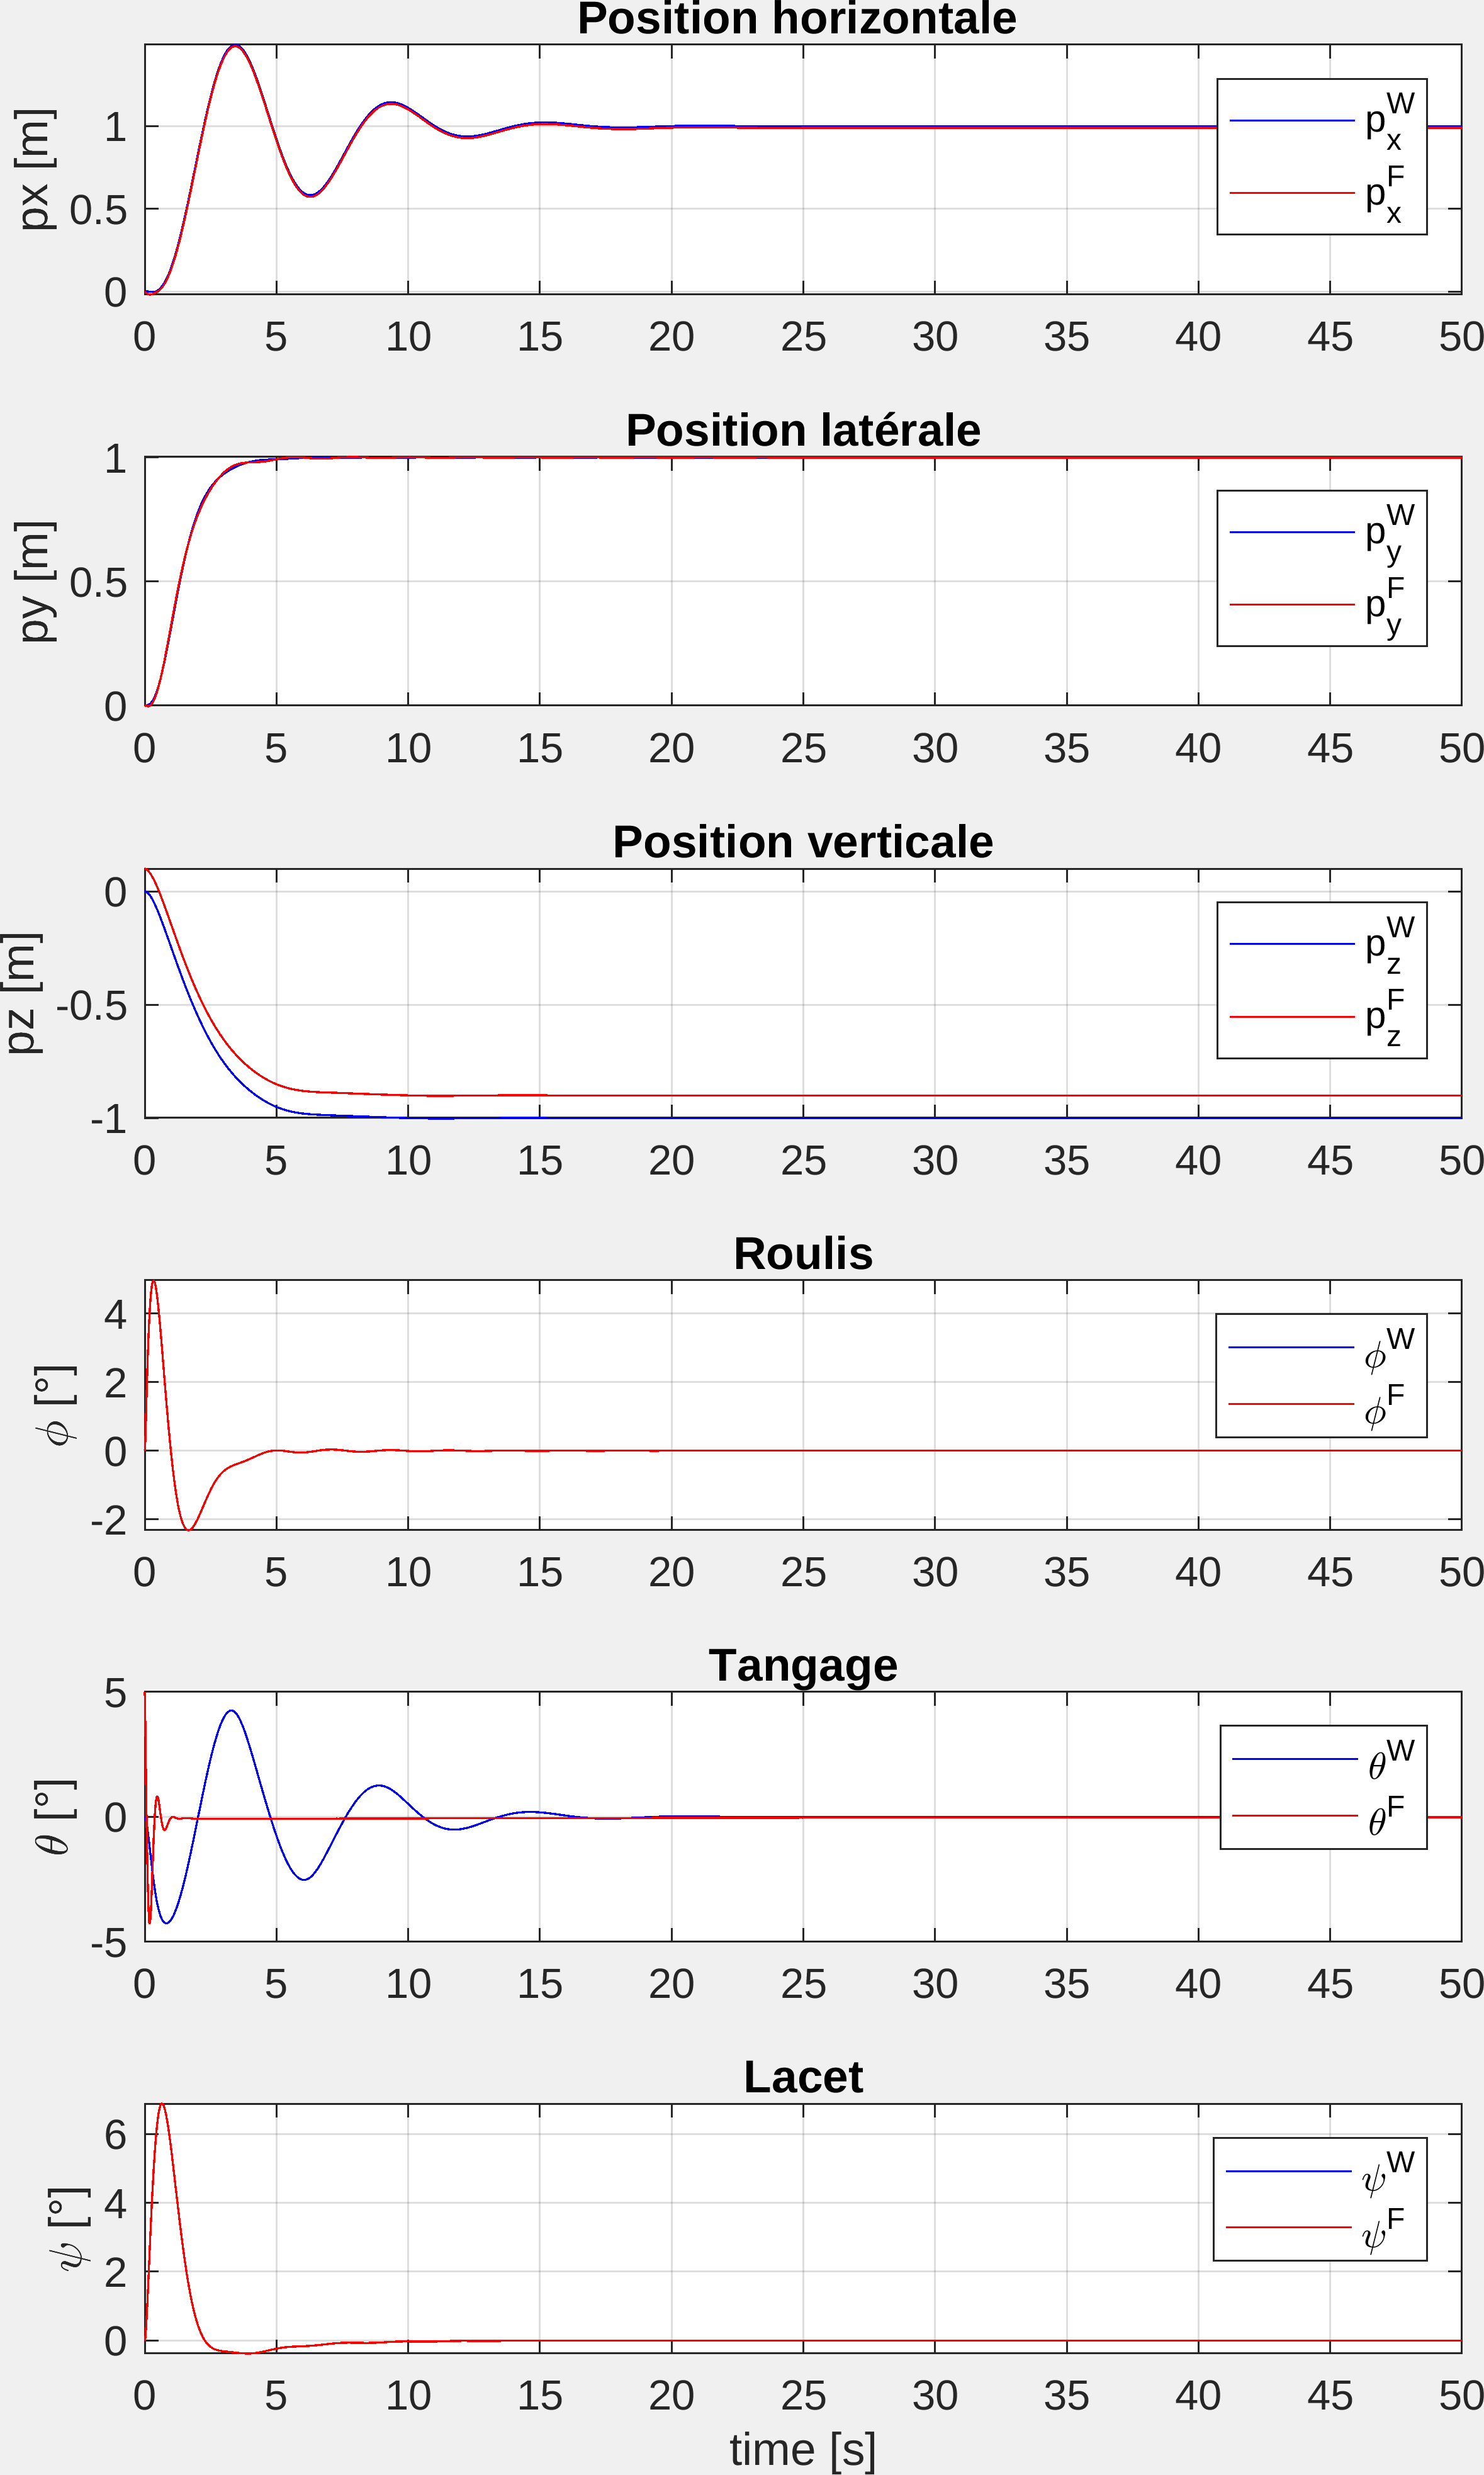
\includegraphics[width=0.6\columnwidth,angle=0]{figures/colibri_sim.png}
    \caption{Simulation de la position et de l'orientation du drone multicorps Colibri en boucle fermée avec un contrôleur à double boucle. }
    \label{fig:sim_colibri}
\end{figure}

En considérant les degrés de liberté de la liaison pivot, le couplage entre les deux corps est clairement visible sur les trois graphiques du bas. En effet, les angles de roulis et de lacet $(\phi_{\text{F}}, \psi_{\text{F}})$ et $(\phi_{\text{W}}, \psi_{\text{W}})$ du fuselage et de l'aile coïncident parfaitement, alors que les angles de tangage $(\theta{\text{F}}, \theta{\text{F}})$ sont différents.








\section{Estimation d'état}\label{sec:stateEst}
% \todo{Link to the modeling:  What is the connection between angular velocity
% estimation and the multibody dynamics derived in the paper?
% What are the advantages of the angular velocity estimator
% compared to existing technologies? It is difficult to
% discern the theoretical contribution to the angular
% velocity estimation part.}


Pour stabiliser ce système de drone à deux corps, il est nécessaire de connaître la position et l'orientation des deux corps. Grâce à la liaison pivot entre l'aile et le fuselage, la différence entre l'orientation de l'aile et l'orientation du fuselage est simplement une rotation autour de l'axe de tangage de l'aile. Les deux autres orientations (roulis et lacet) coïncident. La position du centre de gravité du fuselage peut être déduite de la position du centre de gravité de l'aile et de l'angle entre le fuselage et l'aile. Cet angle est mesuré par un codeur rotatif en quadrature (CUI Devices AMT22, codeurs absolus, 12 bits, SPI), qui renvoie une mesure angulaire quantifiée avec un pas de \SI{0,09}{\degree}. Compte tenu de cette mesure angulaire, nous examinons ci-dessous l'estimation des informations relatives à la vitesse, afin de reconstruire l'état du drone.
\nomenclature[]{\(SPI\)}{Bus de données série synchrone \textit{Serial Peripheral Interface}}

\subsection{Placement des capteurs}
\label{subsec:sens_pos}
Une première question concerne l'emplacement des capteurs : l'IMU (accéléromètre, gyroscope et magnétomètre) peut être installée sur le fuselage ou sur l'aile. 
L'installation de l'IMU sur l'aile permet d'effectuer les mesures directement dans le référentiel souhaité, mais les mesures sont plus bruitées car l'IMU est attachée à la structure supportant les moteurs. Compte tenu de la taille des ailes, leur flexibilité peut générer des résonances et perturber les mesures. 

L'installation de l'IMU sur le fuselage réduit les vibrations, mais implique que les mesures soient transformées dans le référentiel de l'aile. La transformation correspondante peut être calculée à partir de la mesure de l'encodeur rotatif, qui fournit l'angle entre l'aile et le fuselage, ainsi qu'à partir des mesures prises avec le logiciel de CAO, qui fournissent des informations précises sur les distances entre les référentiels de l'aile et du fuselage. Notre choix final est de fixer l'IMU au fuselage. Une autre considération est que la carte de pilotage automatique, qui a déjà une IMU intégrée, est également supposée être connectée à la charge utile et à d'autres capteurs fixés sur fuselage. Il s'agit donc de limiter le nombre de câbles au point de pivot pour les commandes des actionneurs et l'alimentation électrique.

\nomenclature[]{\(CAO\)}{Conception assistée par ordinateur}

\subsection{Estimation de la vitesse angulaire}

Comme expliqué ci-dessus, nous pouvons mesurer l'angle $\kappa \in \real$ entre l'aile et le fuselage à l'aide de l'encodeur rotatif. Ensuite, pour estimer la vitesse angulaire, nous utilisons un observateur grand gain proposé dans \cite{203613} (voir également \cite{1032320} pour l'utilisation d'observateurs grand gain pour estimer les dérivées temporelles). Cette méthode est préférable à une dérivée par différence finie, car les informations quantifiées générées par l'encodeur rotatif peuvent donner lieu à du bruit numérique dans les valeurs estimées de vitesse angulaire.


Désignons par $\kappa \in \real$ l'angle mesuré, par $\omega_{\kappa} := \dot \kappa  \in \real$ sa dérivée à estimer, et par $\xi = [\kappa,~\omega_{\kappa}]^\top \in \mathbb{R}^2$ leur juxtaposition en un seul vecteur. Notons également $\hat{\xi}$ l'estimation de $\xi$ définie par :
%\todo{GH: il y a pas un peu de répétitions dans les notations ?}
%\xi = [\kappa,~\omega_{\kappa}]^\top \in \mathbb{R}^2, \quad 
\begin{align*}
    \hat{\xi} = [\hat{\kappa},~\hat{\omega}_{\kappa}]^\top \in \mathbb{R}^2.
\end{align*}
Suivant \cite{203613}, la dynamique de l'estimateur est donnée par :
\begin{align}
\label{eq:high_dyn}
    \dot{\hat{\xi}} =  \begin{bmatrix}0 & 1 \\ 0 & 0 \end{bmatrix} \hat{\xi}+ \begin{bmatrix}\frac{k_{p}}{\epsilon_{\kappa}}  \\ \frac{k_{v}}{\epsilon_{\kappa}^{2}}  \end{bmatrix} (\kappa - \hat{\kappa}),
\end{align}
où $\kappa$ est la mesure angulaire récupérée du capteur, $k_{p}$ et $k_{v}$ sont deux gains scalaires positifs tels que l'équation caractéristique $s^{2} + k_{v} s + k_{p} = 0$ ait des racines à partie réelle négative. Pour notre estimateur, nous avons choisi $k_{p} = 1$ et $k_{v} = 1,3$ de manière à obtenir un facteur d'amortissement $\zeta = 0,65$ conduisant à une réponse légèrement sous-amortie comme compromis approprié entre un temps de montée rapide et une réponse légèrement oscillatoire. Le gain $\epsilon_{\kappa}$ peut être ajusté de manière pratique afin d'obtenir un compromis entre l'action de lissage (obtenue en augmentant $\epsilon_{\kappa}$) et la réduction du retard temporel
de l'estimateur (obtenue en réduisant $\epsilon_{\kappa}$). En outre, l'action de lissage de l'approche proposée atténue l'effet de la quantification de la mesure angulaire. Nous avons choisi $\epsilon_{\kappa} = 0,05$ pour nos expériences. La Figure~\ref{fig:high_gain} montre les résultats expérimentaux obtenus après la mise en œuvre du filtre grand gain \eqref{eq:high_dyn} dans le cas d'un vol générant des oscillations angulaires de grande amplitude.

Nous avons effectué une dérivation par différence finie (en vert) en post-traitement pour comparer les résultats. En raison de la nature quantifiée de l'encodeur rotatif, nous observons que la vitesse angulaire obtenue par différence finie est très bruitée. On constate que le filtre grand gain permet d'estimer la vitesse angulaire avec plus de précision (en rouge), bien qu'avec un léger retard. Grâce à l'ajout d'une IMU supplémentaire sur l'aile lors d'un essai en vol, il est possible de comparer l'estimation de la vitesse avec les mesures du gyroscope de l'aile (MPU9250), visibles sur le graphique du bas de la Figure~\ref{fig:high_gain} (trace bleue). On constate que les mesures du gyroscope sont quelque peu bruitées, notamment en raison des vibrations générées par les moteurs. 

\begin{figure}[ht!]
\centering
    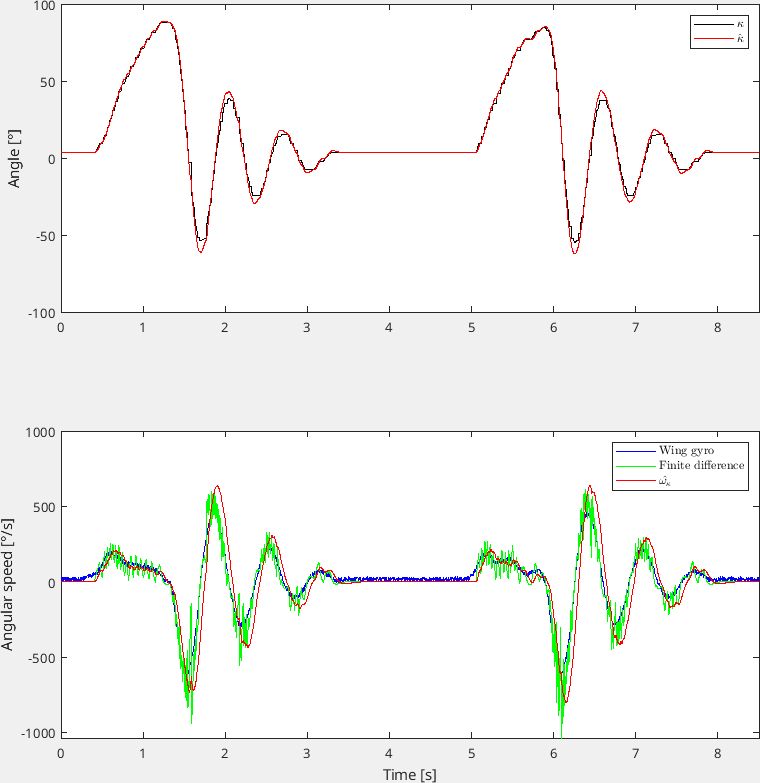
\includegraphics[width=0.6\columnwidth,angle=0]{figures/highGainFilter.png}
    \caption{Mesure de l'angle (noir, graphique du haut), mesure de la vitesse angulaire avec le gyroscope de l'aile (bleu, graphique du bas), estimation de la vitesse angulaire par différence finie (vert, graphique du bas) et estimation avec le filtre grand gain (courbes rouges).}
    \label{fig:high_gain}
\end{figure}
\todo{Ce n'est pas très lisible comme figure}

Afin d'effectuer la transformation nécessaire entre les repères, nous définissons le quaternion $q_{\hat{\kappa}} \in {\mathbb S}^3$ suivant :
\begin{align}
\label{eq:rot_quat}
    q_{\hat{\kappa}} =  \left[\cos\left(\frac{\hat{\kappa}}{2}\right) ~ 0 ~ \sin\left(\frac{\hat{\kappa}}{2}\right) ~ 0 \right]^\top
\end{align}


\subsection{Estimation de l'état de l'aile}

Sur la base de l'angle estimé $\hat{\kappa}$ et de la vitesse angulaire estimée $\hat{\omega}_{\kappa}$, il est possible de transformer les mesures réalisées dans le repère du fuselage vers le repère de l'aile. Tous les capteurs sont installés sur la carte de l'autopilote, qui est elle-même fixée au fuselage. Cependant, nous voulons utiliser INDI pour stabiliser l'aile. Cette loi de contrôle nécessite donc des informations sur l'état du drone dans le repère de l'aile, où toutes les forces sont appliquées (aérodynamiques et de traction).
Deux solutions viables sont alors possibles : effectuer l'estimation d'état dans le repère du fuselage et faire pivoter l'estimation en utilisant l'estimation de l'angle $\hat{\kappa}$, ou faire pivoter les mesures brutes à l'avance pour les exprimer dans le repère l'aile, et ensuite effectuer l'estimation d'état dans ce dernier. 
Compte tenu de l'architecture actuelle du logiciel du système Paparazzi (voir Annexe \ref{sec:logiciel}), il est impossible d'avoir deux structures conjointes d'estimation de l'état. Il est donc complexe de mettre en œuvre la première solution, dans laquelle le contrôleur récupère directement l'estimation de l'état actuel. C'est pourquoi nous avons choisi d'estimer l'état de l'aile à partir des données mesurées sur le fuselage. À cette fin, nous détaillons ci-dessous les transformations pour les trois capteurs : gyroscope, accéléromètre et magnétomètre. 

Pour les mesures de la vitesse angulaire basées sur le gyroscope, nous pouvons calculer la vitesse angulaire de l'aile exprimée dans le repère de l'aile :
\begin{align}
    \label{eq:gyro_deplacement}
    \omega_{\text{W}} = R(q_{\hat{\kappa}}) \left( \omega_{gyro}^{\text{F}} + \begin{bmatrix}
    0\\ \omega_{\kappa} \\ 0
    \end{bmatrix}  \right) 
\end{align}
où $\omega_{gyro}^{\text{F}}$ est la vitesse angulaire mesurée par le gyroscope sur le fuselage, exprimée dans le repère du fuselage, $\hat{\omega}_{\kappa}$ est la vitesse angulaire estimée de l'aile par rapport au fuselage, conformément à \eqref{eq:high_dyn}, et $q_{\hat{\kappa}}$ est le quaternion défini dans \eqref{eq:rot_quat}.
L'expression \eqref{eq:gyro_deplacement} est similaire à une composition de vitesse angulaire et à un changement du repère.

Pour la mesure de l'accélération avec l'accéléromètre, nous pouvons utiliser la relation de l'équation \eqref{eq:accel_deplacement}, qui est obtenue à partir du théorème de transport du taux de variation \cite{brizard2004motion}, où nous trouvons le terme d'accélération d'Euler $\dot{\omega_{\text{F}}} \times d_{AF}$  et le terme d'accélération centripète $\omega_{\text{F}} \times ( \omega_{\text{F}} \times  d_{AF})$. L'accélération de Coriolis $2\omega_{\text{F}} \times \frac{d (d_{\text{FW}})}{d t}\Bigr|_{O_{\text{F}}}$ et le taux d'accélération $\frac{d^{2} (d_{\text{FW}})}{d^{2} t}\Bigr|_{O_{\text{F}}}$ sont nuls car $d_{\text{FW}}$ est constant.

\begin{align}
    \label{eq:accel_deplacement}
    a_{\text{W}} = R(q_{\hat{\kappa}}) \left( a_{acc}^{F} + \dot{\omega}_{gyro}^{F} \times d_{\text{FW}} + \omega_{gyro}^{F} \times ( \omega_{gyro}^{F} \times  d_{\text{FW}}) \right) 
\end{align}
où $a_{acc}^{F} \in \real^{3}$ est l'accélération mesurée par l'accéléromètre sur le fuselage, exprimée dans le repère du fuselage et $\omega_{gyro}^{F}$ est la vitesse angulaire du fuselage, identique à l'équation \eqref{eq:gyro_deplacement}. L'accélération angulaire $\dot{\omega}_{gyro}^{F}$ dans \eqref{eq:accel_deplacement} est calculée par différence finie.


Pour les mesures du magnétomètre, nous avons :
\begin{align}
    \label{eq:mag_deplacement}
    E_{\text{W}} = R(q_{\hat{\kappa}}) E_{mag}
\end{align}
où $E_{mag} \in \real^{3}$ est la sortie du magnétomètre, exprimée dans le repère du fuselage et $ E_{\text{W}} \in \real^{3}$ est la mesure exprimée dans le repère de l'aile.

Pour obtenir une estimation de l'état de l'aile, nous utilisons un algorithme de fusion des mesures des capteurs : le filtre de Kalman étendu (EKF)  \nomenclature[]{\(EKF\)}{Filtre de Kalman étendu (\textit{Extended Kalman Filter})} qui fournit une estimation des états suivants : $p_{\text{W}}$, $v_{\text{W}}$, $q_{\text{W}}$ à partir de mesures transformées dans le repère de l'aile $\omega_{\text{W}}$ (équation \eqref{eq:gyro_deplacement}), $a_{\text{W}}$ (équation \eqref{eq:accel_deplacement}), $E_{\text{W}}$ (équation \eqref{eq:mag_deplacement}) et les données du système de vision externe, qui fournissent une mesure précise de la position $p_{text{W}}$ et de la vitesse $v_{text{W}}$ du drone dans le repère inertiel (I).


\subsection{Estimation de l'orientation du fuselage}
Pour déterminer l'orientation du fuselage, nous pouvons effectuer une composition entre le quaternion représentant l'orientation de l'aile $q_{text{W}}$ résultat de l'EKF et le quaternion construit à partir de la mesure filtrée de l'encodeur rotatif $q_{\hat{\kappa}}$ dans \eqref{eq:rot_quat},
\begin{align}
\label{eq:quat_fuselage}
    q_{\text{F}} = q_{\text{W}} \otimes q_{\hat{\kappa}}
\end{align}
où l'opérateur $\otimes$ désigne le produit hamiltonien. La connaissance de $q_{\text{F}}$ est nécessaire pour maintenir le fuselage parfaitement horizontal. 

\section{Inversion non linéaire incrémentale de la dynamique du drone}

\todo{Détails}
La théorie de l'inversion dynamique non linéaire incrémentale (INDI) utilisée dans le contexte des micro-drones est présentée dans \cite{smeurINDI}. Nous utilisons la notation proposée dans \cite{smeurINDITail}. L'hypothèse centrale sous-jacente est que le principe de séparation des échelles de temps s'applique à la dynamique de l'actionneur et à la dynamique des forces et des moments aérodynamiques. Le signal de commande peut alors être calculé de manière incrémentale en utilisant la matrice d'efficacité de l'actionneur $G$.

\begin{align}
    u_{\text{W}} = u_{\text{W}} + G^{\dag} (\nu - \begin{bmatrix}
    \dot{\omega}_{\text{W}} \\
    T_{\text{W}}
    \end{bmatrix})
\end{align}
\todo{$\nu$ explication}
où  $ \dot{\omega}_{\text{W}} \in \real^{3}$ est l'accélération angulaire obtenue par différence finie à partir de l'équation \eqref{eq:gyro_deplacement},  $T_{\text{W}} \in \real$ est la poussée actuelle, $\nu$ est défini dans \cite[équation (4)]{smeurINDITail} et $G$ est la matrice d'efficacité du contrôle, défini par :
\begin{align*}
    \begin{bmatrix}
    \partial \phi \\
    \partial \theta \\
    \partial \psi \\
    \partial T
    \end{bmatrix}\! =\! G u_{f} \!=\!
    \begin{bmatrix}
    -7.5 & -15 & 7.5 & 15 & 0 & 0\\
    0 & 0 & 0 & 0 & 15 & 15 \\
    0 & 0 & 0 & 0 & 4 & -4 \\
    -0.6 & -0.6 & -0.6 & -0.6 & 0 & 0\\
    \end{bmatrix}
    u_{f}
\end{align*}
Cette sélection de la matrice d'efficacité a été déterminée pour les vols stationnaires, mais il est nécessaire d'effectuer une étude différente pour le vol vers l'avant.

Pour stabiliser le fuselage, nous utilisons un bouclage proportionnel-dérivé de l'angle $\theta_{\text{F}}$ formé entre le fuselage et l'horizontale, que nous voulons maintenir à zéro. Cet angle est obtenu en convertissant le quaternion $q_{\text{F}}$ de l'équation \eqref{eq:quat_fuselage} en un angle d'Euler en suivant la convention d'Euler 'ZYX'. Le bouclage fournit la commande $u_{text{tail}}$ pour la vitesse angulaire du moteur générant la force $F_{m}$ (voir Figure~\ref{fig:colibri_frame_side}), suivant l'expression :
\begin{align*}
    u_{\text{tail}} = u_{eq} + k_{p} \theta_{\text{F}} + k_{d} \dot{\theta_{\text{F}}},
\end{align*}
où $u_{eq}$ est la commande, à l'équilibre, du moteur pour maintenir le fuselage horizontal en l'absence de perturbation et $k_{p}$, $k_{d}$ sont des gains scalaires ajustables. La valeur $u_{eq}$ a été obtenue en appliquant le théorème des moments au fuselage au point $O_{\text{W}}$. En effet, les deux moments qui agissent sur le fuselage sont le couple dû à la force de poussée du moteur et le couple dû à la position du centre de gravité du fuselage.
\todo{Expliquer les moments}

Les gains $k_{p}$ et $k_{d}$ ont été ajustés en vol pour assurer un comportement satisfaisant. On obtient $\dot{\theta_{\text{F}}}$ à partir de $\omega_{gyro}^{F} = [\dot{\phi_{\text{F}}}~\dot{\theta_{\text{F}}}~\dot{\psi_{\text{F}}}]^\top$.

\section{Expérimentations}
\label{sec:exp}
% \todo{Photo de la volière: It is difficult to understand the experimental results
% due to the absence of snapshots, detailed explanations, or
% pictures of the experimental environment. Illustrations and
% explanations of the experimental structure, actual flight
% photos, and the design structure of the entire flight
% system must be added.}
Un prototype a été mis au point, comme le montre la Figure~\ref{fig:colibri_real}. La Figure~\ref{fig:colibri_flight} présente une sélection des résultats expérimentaux en environnement contrôlé.


\begin{figure}[ht!]
    \centering
    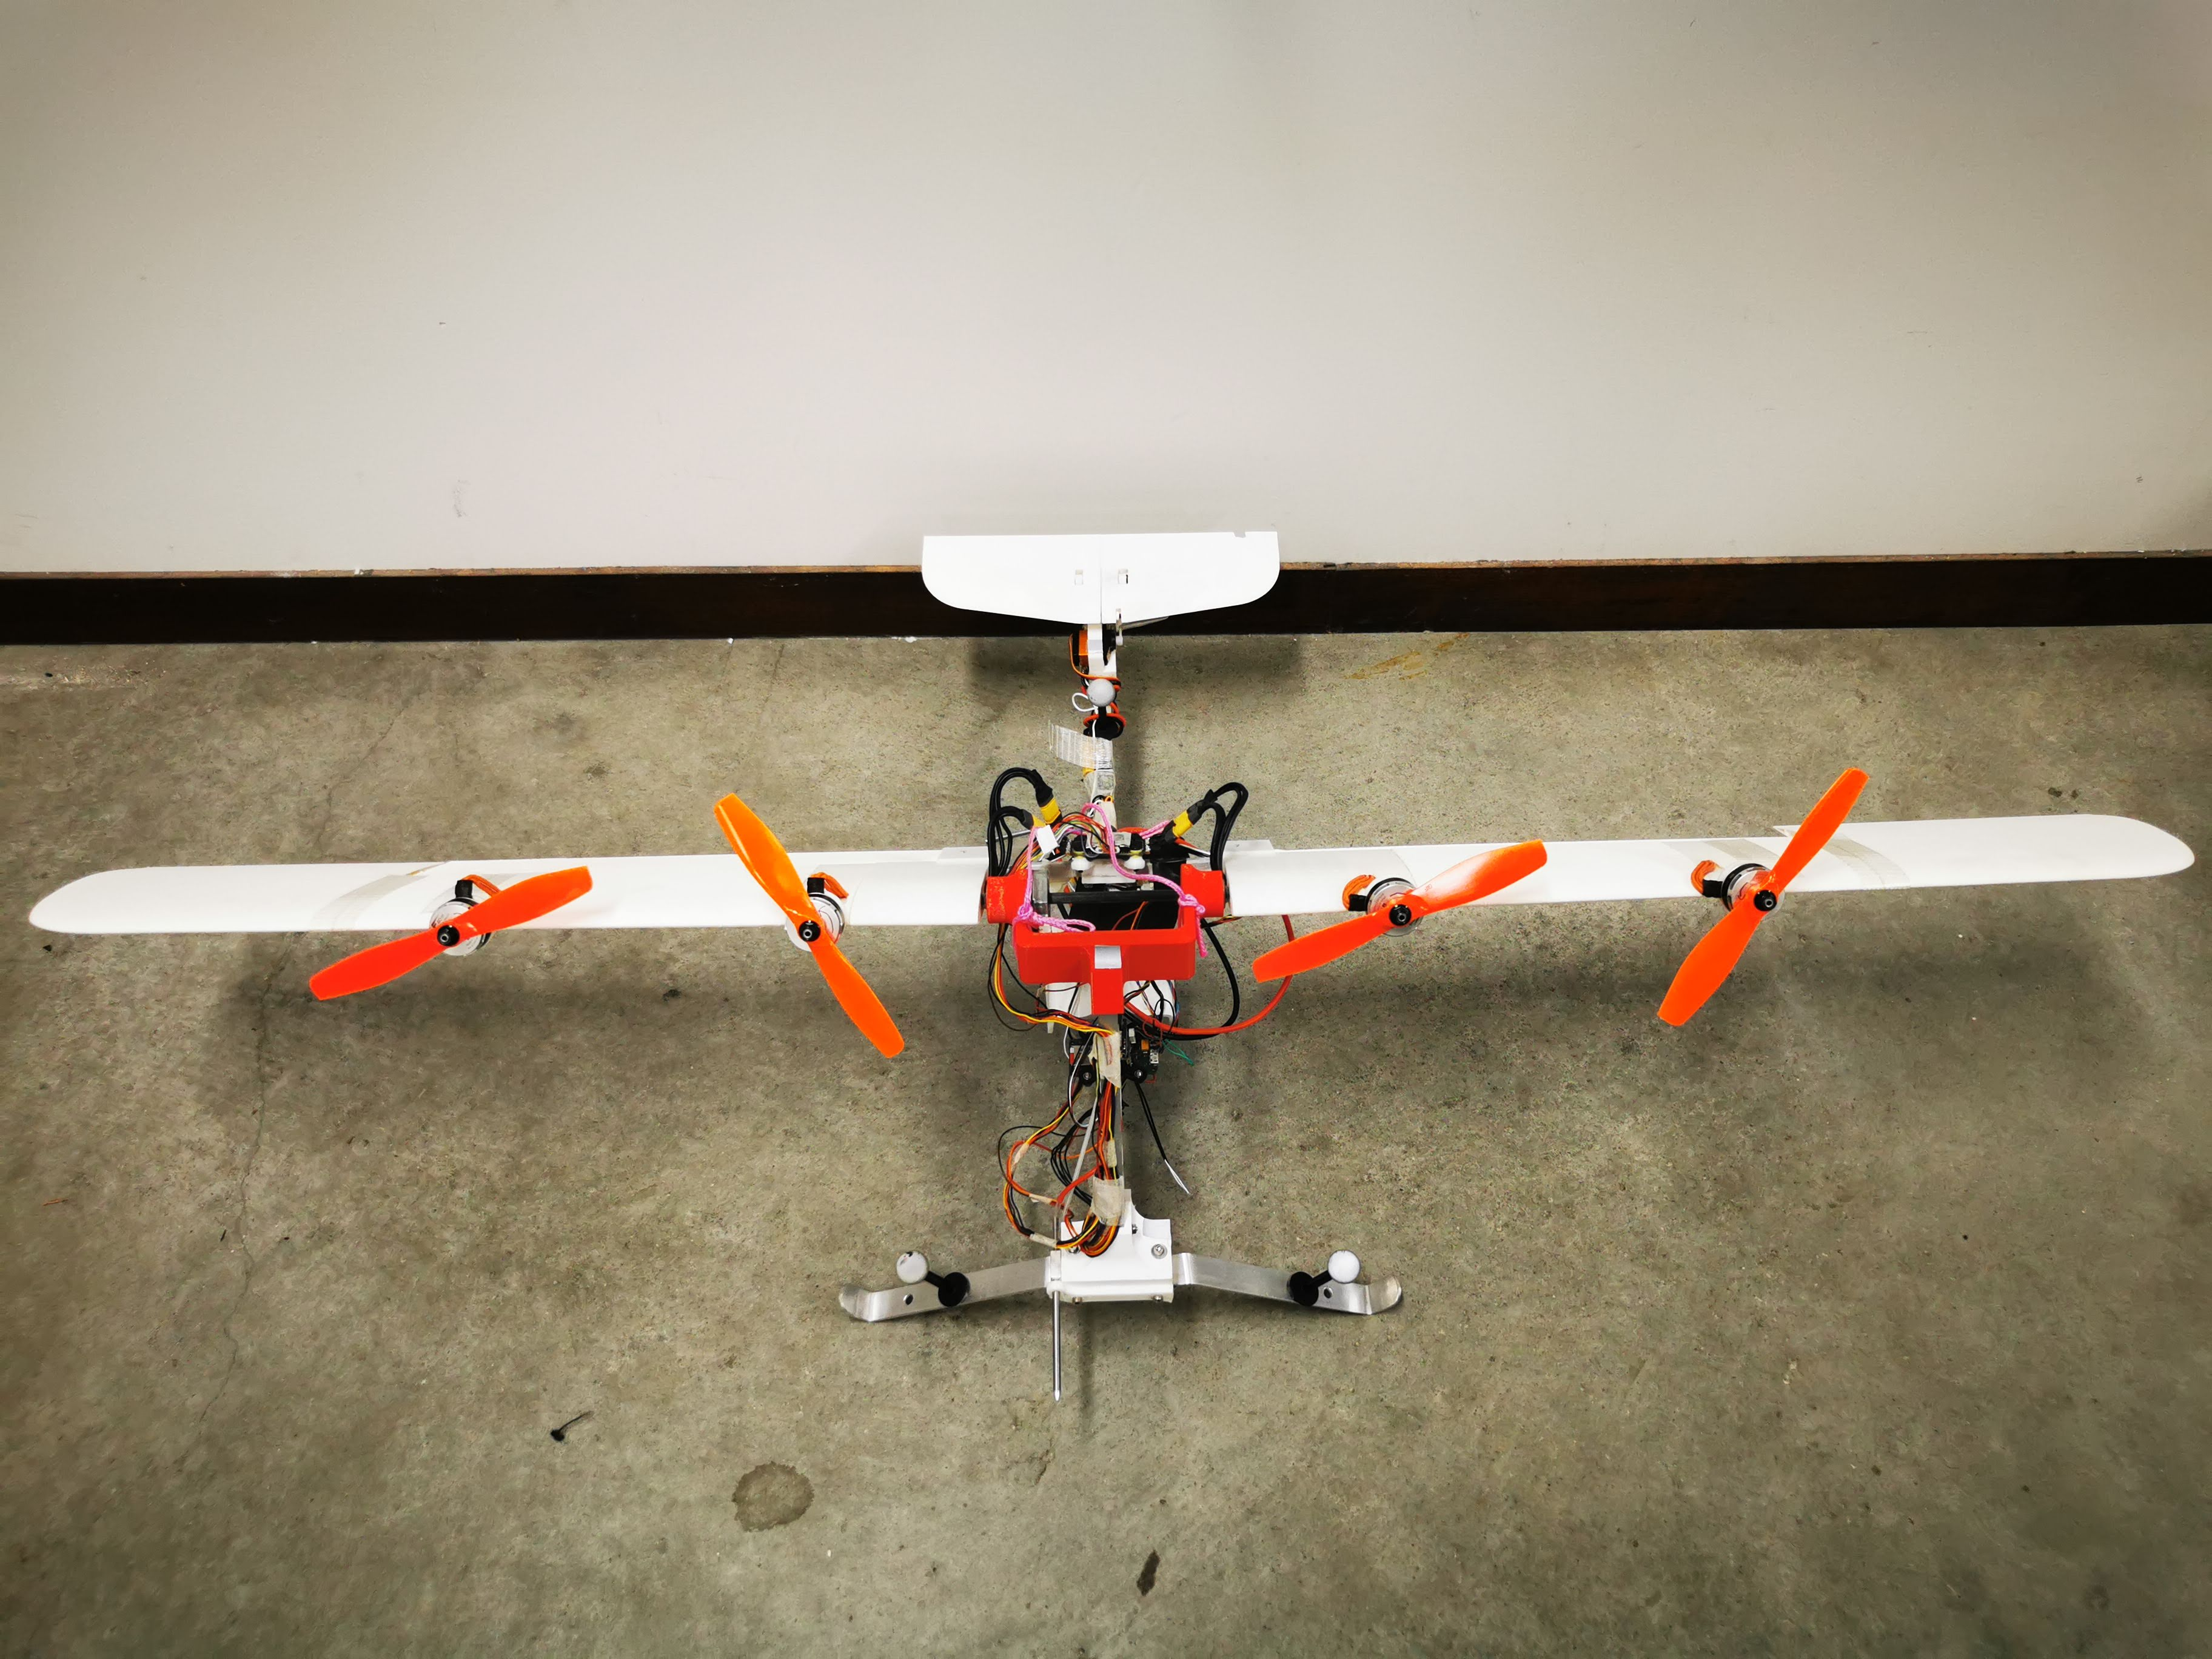
\includegraphics[trim={0 15cm 0 25cm},clip, width=0.6\columnwidth]{figures/colibri_real.jpg}
    \caption{Prototype : Colibri.}
    \label{fig:colibri_real}
\end{figure}

Sur la Figure~\ref{fig:colibri_flight}, de \SI{0}{\second} à \SI{8}{\second}, le drone est au sol. De \SI{8}{\second} à \SI{16}{\second}, le drone décolle pour atteindre une hauteur de 2 mètres, visible sur le troisième graphique. Cette hauteur est atteinte après un dépassement de 10 \%. Le drone est maintenu dans cette position pendant \SI{54}{\second}. Des oscillations d'incidence sont observées dans le cinquième et le dernier graphique, générant des oscillations dans la position horizontale du drone. Ce phénomène est dû au couplage entre les deux corps, qui n'est pas correctement stabilisé. À partir de \SI{70}{\second}, le drone commence à se diriger vers le point $p_{c} = \begin{bmatrix} 3 & 0.9 & -1.5 \end{bmatrix}^\top$ et $\psi_{c}=\SI{90}{\degree}$.
\begin{figure}[ht!]
\centering
    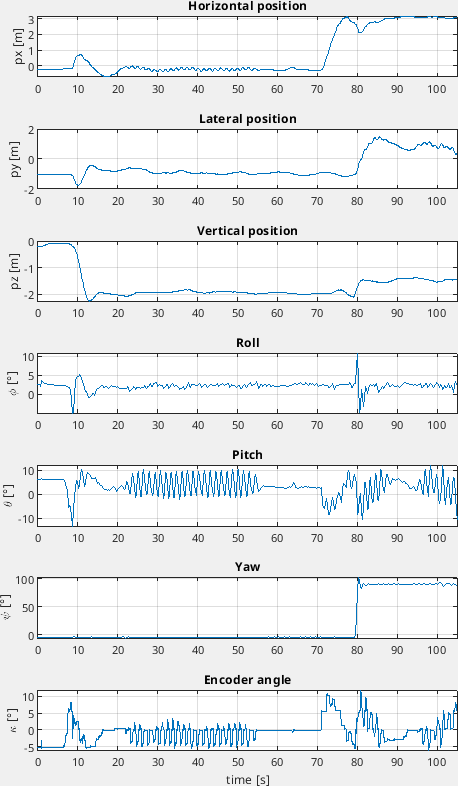
\includegraphics[width=0.6\columnwidth,angle=0]{figures/colibri_flight.png}
    \caption{Position et orientation de l'aile dans les six premiers graphiques et mesure de l'angle entre l'aile et le fuselage sur le dernier graphique lors d'un vol réel. }
    \label{fig:colibri_flight}
\end{figure}

\section{Vol avec un contrôleur unifié}

\section{Commande Udwadia-Kalaba}

Mesure du vent, sonde 5 trous

\section{Vols expérimentaux}

\section{Conclusion du Chapitre \ref{chap:colibri}}






